\chapter{Das Programm}\label{the_program}

In diesem Kapitel werden wir auf die Implementierung von Netzwerk \ref{net_sltr} aus dem vorherigen Abschnitt eingehen. Das im Folgenden beschriebene Programm baut auf Vermutung \ref{int_conj} -- dass sich aus jedem nicht ganzzahligen zulässigen Fluss auf Netzwerk \ref{net_sltr} ein Gutes-FAA extrahieren lässt -- auf. Der Code wurde in SageMath geschrieben und ist auf Anfrage erhältlich \cite{sage}. Algorithmus \ref{algo_gfaa} gibt einen Überblick der durchgeführten Schritte bei der Suche nach einem Guten-FAA für einen gegebenen ebenen intern-3-zusammenhängenden Graphen mit Aufhängungen $\{a_1,a_2,a_3\}$

\begin{algorithm}
\caption{Berechnung eines Guten-FAA}
\label{algo_gfaa}
\begin{algorithmic}[1]
\Procedure{GFAA}{$G,f_{aus},\{a_1,a_2,a_3\}$}
\If{FAA$(G,\{a_1,a_2,a_3\}) \neq$ None}	
	\State $\{d_1,d_2\} \gets $ demands for $\mathcal{N}_G$
	\State initialize $\mathcal{N}_G$\Comment nach Netzwerk \ref{net_sltr}
	\State $\varphi=(\varphi_1,\varphi_2) \gets $ two-flow$(\mathcal{N}_G)$\label{two_flow1}
	\If {$\varphi \neq$ None}
		\If{$\varphi$ is integer}
			\State $\phi \gets $ FAA$(\varphi_2)$
			\State \Return $\phi$
		\Else
			\State $\varphi_z \gets$ FAA-flow($\varphi_2$)\Comment Fluss nach Proposition \ref{lem_faa}
			\State $\mathcal{N} \gets \mathcal{N}_G \backslash \{$edges used by $\varphi_z\}$\label{algo_check}
			\State $\tilde{\varphi} \gets $ int-one-flow$(\mathcal{N})$\Comment Ecken- und Schnyder-Fluss zu $\varphi_z$\label{int_one_flow1}
			\If { $|\tilde{\varphi}| = d_1+d_2-|\varphi_z|$ }
				\State $\phi \gets $ FAA$(\varphi_z)$
				\State \Return $\phi$
			\Else \Comment Nur erreichbar, falls Vermutung \ref{faa_conj} falsch\label{sanity_check}
				\State $\varphi=(\varphi_1,\varphi_2) \gets $ int-two-flow$(\mathcal{N}_G)$
				\If {$\varphi \neq$ None}\Comment Sonst Gegenbeispiel zu Vermutung\ref{int_conj}\label{int_two_flow1}
					\State $\phi \gets $ FAA$(\varphi_2)$
					\State \Return $\phi$
				\EndIf
			\EndIf
		\EndIf
	\EndIf
\EndIf
\EndProcedure
\end{algorithmic}
\end{algorithm}


Die Kontrolle, ob für $G$ ein FAA existiert ist optional, lässt sich jedoch, zum Beispiel wie zuvor über ein 1-Fluss-Problem, in polynomineller Zeit auf einem deutlich kleineren Netzwerk bestimmen. Dies spart Zeit, falls zu Aufhängungen keine FAAs auf $G$ existieren. Das Multi-Fluss-Problem auf $\mathcal{N}_G$ zu gegebenen Bedarfen $(d_1,d_2)$ wird mithilfe des in SageMath enthaltenen Solvers \textit{Glpk} für Lineare Programmierung gelöst, welcher ein Paar von Flussgraphen $(\varphi_1,\varphi_2)$ ausgibt, falls eine zulässige Lösung existiert und sonst nichts\cite{glpk,sage}. In den Zeilen \ref{int_one_flow1} und \ref{int_two_flow1}, wird im Gegensatz zu Zeile \ref{two_flow1}, nur nach ganzzahligen Lösungen gesucht. Aus einer ganzzahligen Lösung kann man ein FAA $\phi$ aus $\varphi_2$ extrahieren indem man die Zuweisungs-Pfade durch die Dummy-Senke zurück verfolgt. Wir betreten jeden passierten Dummy-Knoten $v^*$ aus einem Winkel $(f,v)$. Diese Winkel ergeben die Zuweisungen $\phi$.

Die Überprüfung ab Zeile \ref{algo_check} ist unter der Annahme, dass Vermutung \ref{int_conj} stimmt nicht notwendig. Es könnte hier ein FAA aus $\varphi_2$ extrahiert und ausgegeben werden. Wir gewährleisten  jedoch so die Korrektheit des Algorithmus, weil wir den Beweis von Vermutung \ref{int_conj} noch nicht gefunden haben. Bei Tests ergaben sich mit diesem Ansatz kürzere Berechnungszeiten, als bei der Suche nach ausschließlich ganzzahligen Lösungen. Zeile \ref{sanity_check} sollte nach Vermutung \ref{int_conj} nicht erreicht werden. Sie stellt jedoch sicher, dass Algorithmus \ref{algo_gfaa} immer dann ein Gutes-FAA ausgibt, wenn ein ganzzahliger Fluss auf Netzwerk \ref{net_sltr} existiert.

\begin{remark}
In der Implementierung wurden die Kanten innerhalb von Gebieten $f$ mit $|3|=3$ weggelassen, da die einzig mögliche Lösung hier ist, dass nur drei Ecken-Pfade durch das Gebiet laufen. Die Bedarfe werden dementsprechend angepasst.
\end{remark}

\section{Visualisierung}

Nehmen wir an, wir haben für einen Graphen $G$ ein Gutes-FAA $\phi$ gefunden. Für eine SLTR, müssen wir eine zu $\phi$ passende Einbettung von $G$ finden. Wir werden den in Abschnitt \ref{harmonic_approach} erörterten Ansatz über harmonische Funktionen nutzen, um eine SLTR von $G$ zu erhalten.

Wir wollen nun eine Einbettung $f:V\to \mathbb{R}^2$ von $G$ ähnlich der Gummiband-Repräsentation berechnen, die $\phi$ respektiert. Sei $S \subseteq V$ die Menge der Knoten von $f_{aus}$. Nach Abschnitt \ref{harmonic_approach} gelten die folgenden harmonischen Gleichungen für zugewiesene (oben) und nicht zugewiesene Knoten (unten).
$$ f(v) = \lambda_v f(u) + (1-\lambda_v)f(w) \text{, mit } \lambda_v \in (0,1) $$
$$ f(v) = \sum_{u \in N(v)} \lambda_{uv} f(u) \text{, mit }  \sum_{u \in N(v)}\lambda_{uv} = 1 \text{ und } \lambda_{uv} > 0 $$
Um zu einer gegebenen Gewichtsfunktion $\lambda$ eine Lösung zu finden, können wir diese Gleichungen, um die Aufhängungen $A = \{a_1,a_2,a_3\}$ erweitern und als Matrix schreiben.
\[ M_{\lambda}(\vec{v_x},\vec{v_y}) = \big( \begin{smallmatrix}f(A)_x&f(A)_y\\ 0&0\end{smallmatrix} \big) \text{, mit } (M_{\lambda})_{vw} =
	\begin{dcases}
	-\lambda_{vw} & \text{falls } (v,w) \in E, \\
	\textstyle\sum_{u \in N(v)} \lambda_{uv} & \text{falls } v = w, \\
	0 & \text{sonst.} \\
	\end{dcases}
\]
Wenn wir nun die Pseudo-Inverse berechnen, erhalten wir eine Einbettung.
$$f(V) = M_{\lambda}^{-1}\big( \begin{smallmatrix}f(A)_x&f(A)_y\\ 0&0\end{smallmatrix} \big).$$
Wir wollen nun, inspiriert von den \textit{iterativen Tutte Einbettungen} nach Felsner und Scheucher, diese Rechnung mehrmals durchführen und Schritt für Schritt die Gewichtung $\lambda$ anpassen \cite{fs17}. Wünschenswert wäre es, wenn sich die Zeichnung nach einer gewissen Anzahl an Schritten nur noch so wenig verändert, dass wir den Algorithmus abbrechen können, und die letzte Zeichnung ausgeben.

\subsection{Probleme bei der Wahl von $\lambda$}

Setzten wir im ersten Durchlauf $\lambda = 1$ erhalten wir eine klassische Gummiband-Repräsentation die $\phi$ respektiert. Wir wollen nun anhand dieser Einbettung $\lambda$ verändern um, Iteration für Iteration, eine \glqq schönere\grqq{ } Einbettung zu erhalten. Halten wir zwei Punkte fest, die wir als Bewertungsmaßstab für eine schöne Einbettung berücksichtigen können.
\begin{itemize}
\item Es gibt keine zu großen oder zu kleinen Gebiete.
\item Es existieren keine zu kurzen Kanten.
\end{itemize}

Sehr lange Kanten lassen sich, wie in Beispiel \ref{bsp_large_corner}, nicht immer vermeiden. Es gibt SLTRs, wie in Beispiel \ref{bsp_long_segment}, bei denen alle inneren Knoten zugewiesen sind. Dies macht eine gute Wahl der $\lambda$ kompliziert. Der Ansatz nach Scheucher \cite{fs17}, bei dem $\lambda$ als monoton steigende Funktion, proportional zu Größe der an eine Kante angrenzenden Gebiete und ihrer Länge gewählt wird, konvergiert im Allgemeinen nicht und liefert so auch keine schönen Zeichnungen. Allgemein wurden besonders SLTRs mit wenigen Kanten betrachtet, da für diese die oben erwähnten Einschränkungen stärker auftreten.

\begin{example}\label{bsp_long_segment}
Bei der in Abbildung \ref{long_segment} a) zu sehenden SLTR sind alle Knoten bis auf die Aufhängungen einem Gebiet zugeordnet. Somit liegt jeder Knoten auf einer Gerade und es existieren nur Gleichungen von Typ
$$ f(v) = \lambda_v f(u) + (1-\lambda_v)f(w) \text{, mit } \lambda_v \in (0,1).$$
Um von der linken zur rechten Zeichnung zu gelangen, wollen wir das Gebiet unten in der Mitte verkleinern, doch die drei angrenzenden Kanten kommen in keiner der Gleichungen zu Bestimmung unserer Einbettung $f(V)$ vor. Die Kanten die uns helfen können, das Segment in rot nach unten zu bewegen und somit das untere Dreieck zu verkleinern, sind in blau eingefärbt. Um zur Zeichnung auf der rechten Seite zu gelangen, erfolgt die Wahl der $\lambda$ in jedem Schritt nach folgenden Schema. Wir berechnen zu jedem Segment die Mengen der Kanten $S_1,S_2$, die an Gebieten liegen die vollständig auf einer der beiden Seiten des Segments liegen. Parallel dazu berechnen wir die Summe der Flächen dieser Gebiete $A_1,A_2$. Falls beide Mengen nicht leer sind erhöhen wir für jede Kante $e \in A_i$ $\lambda(e)$ um $a_i$ mit:
$$ a_i = A_i^{1.25}*|A_j|^{-2} \text{ , mit } j \neq i.$$
Die Exponenten sind heuristisch gewählt. Wir brechen entweder ab, wenn die Einbettung konvergiert oder wir eine feste Anzahl an Schritten durchgeführt haben. Eine so errechnete Einbettungen ist in Abbildung \ref{long_segment} c) zu sehen.
\end{example}

\begin{figure}[h]
	\centering
  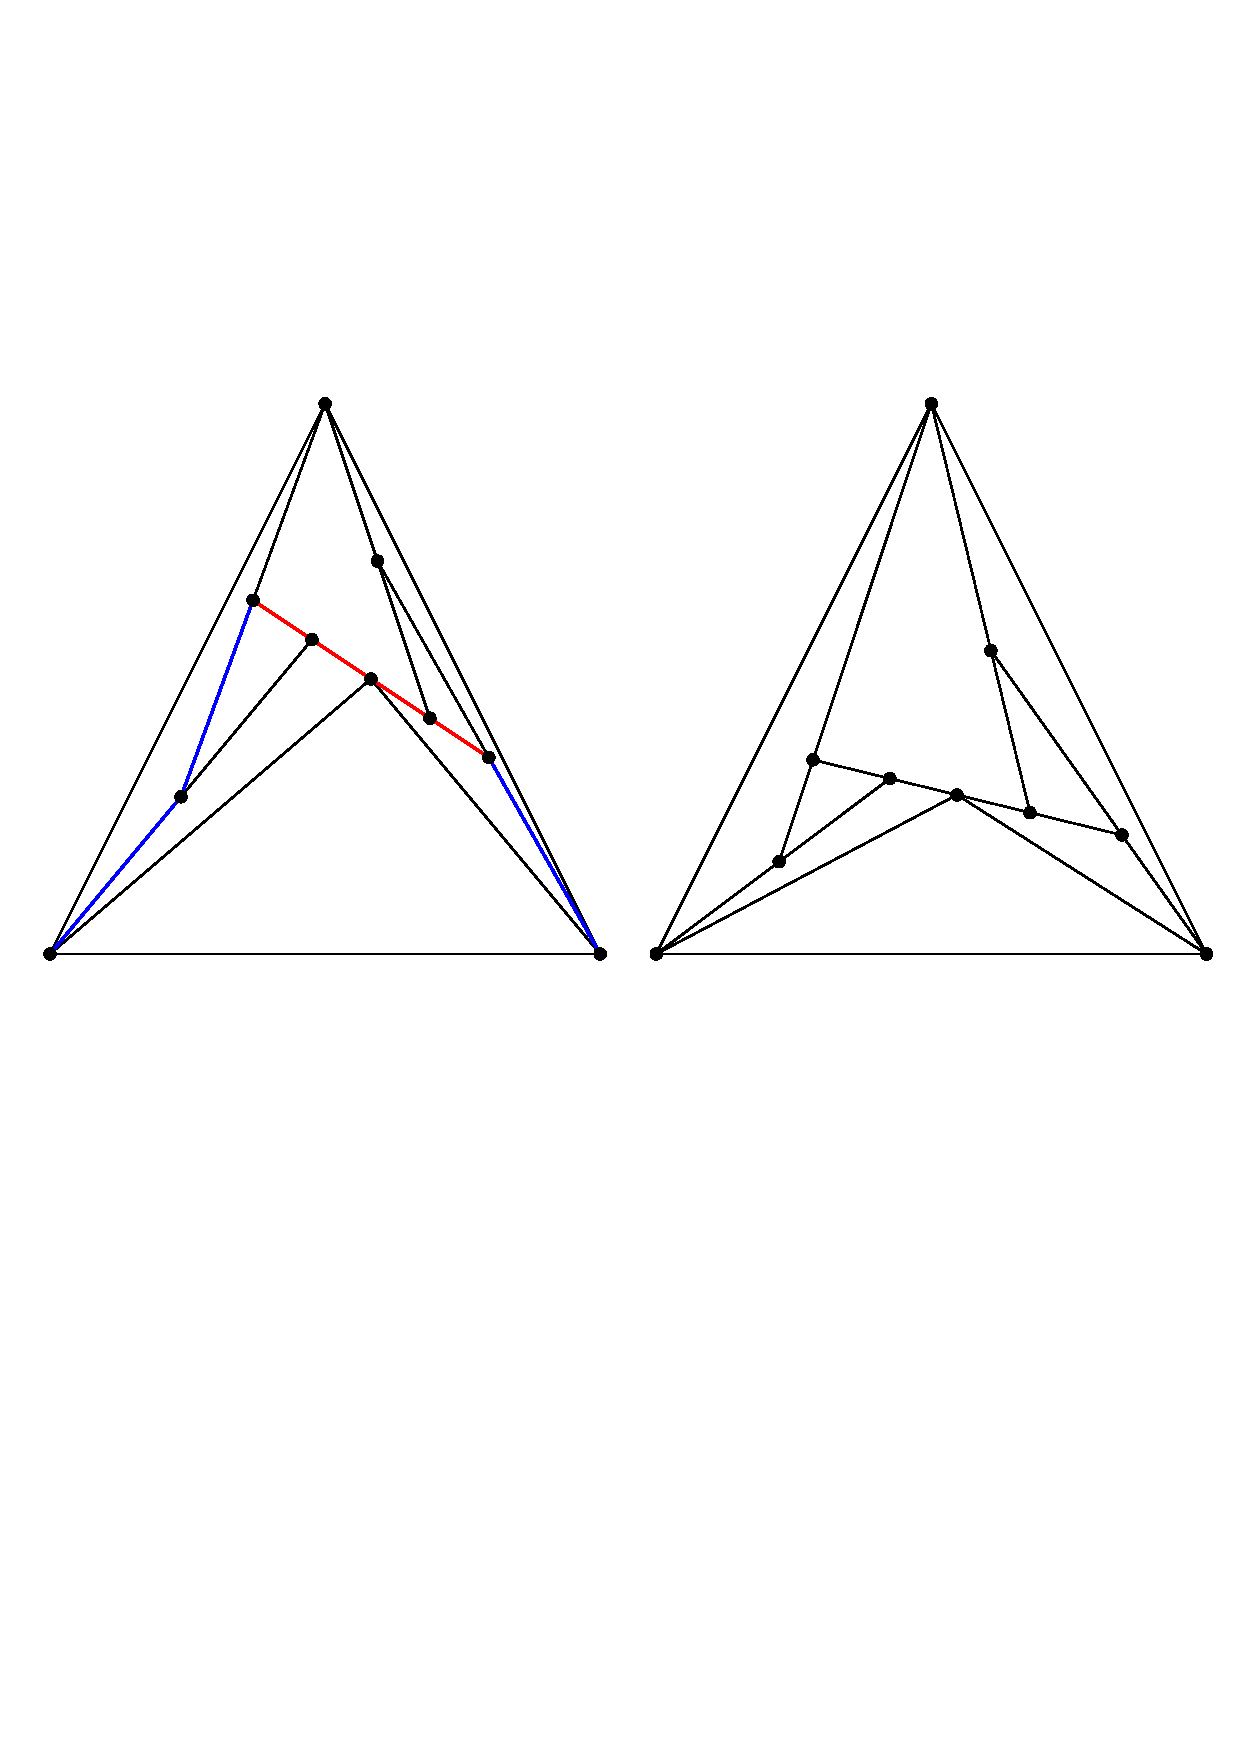
\includegraphics[width=1\textwidth]{example1_vis.pdf}
  \caption{a) Eine Einbettung mit $\lambda$=1. b) Eine Einbettung nach bei der wir nur zu $e$ adjazente Gebiete für $\lambda(e)$ berücksichtigen. c) Eine Einbettung nach dem Schema aus Beispiel \ref{bsp_large_corner}.}
  \label{long_segment}
\end{figure}

Dieser Ansatz führt aber, gerade bei Graphen mit vielen Knoten, zu keiner Zeichnung die die oben genannten Punkte erfüllt (vergleiche Abbildung \ref{large_corner}, b)). Wir betrachten ein weiteres Beispiel um ein zweites Schema zu erläutern.

\begin{example}\label{bsp_large_corner} 
Gerade für Graphen mit vielen Knoten führt der Ansatz aus Beispiel \ref{bsp_long_segment} nicht immer zu einer schönen Zeichnung der SLTR. In Abbildung \ref{large_corner} a) ist so ein Graph mit der ersten, für $\lambda=1$, erhaltenen Zeichnung und dem Resultat nach 50 Schritten nach dem Schema aus Beispiel \ref{bsp_long_segment} zu sehen (Abbildung \ref{large_corner} b). Ein anderer iterativer Ansatz führt hier jedoch zu schöneren Ergebnissen. Wir setzen bei der Initialisierung $\lambda_0(e)=2$ für jede Kante von $G$. Nun multiplizieren wir die Kanten an den Gebieten $f$ mit $A(f) > A(f_{max})*(1+\epsilon)$ mit einer Konstante $c \in \mathbb{N}$. Für diese Kanten gilt somit $\lambda_{i+1}(e) = \lambda_{i}(e)*c$. Wir wählen $\epsilon = 0,1$ und $c=2$. In Abbildung \ref{large_corner} c) ist die Einbettung nach 50 Schritten zu sehen.
\end{example}

\begin{figure}[h]
	\centering
  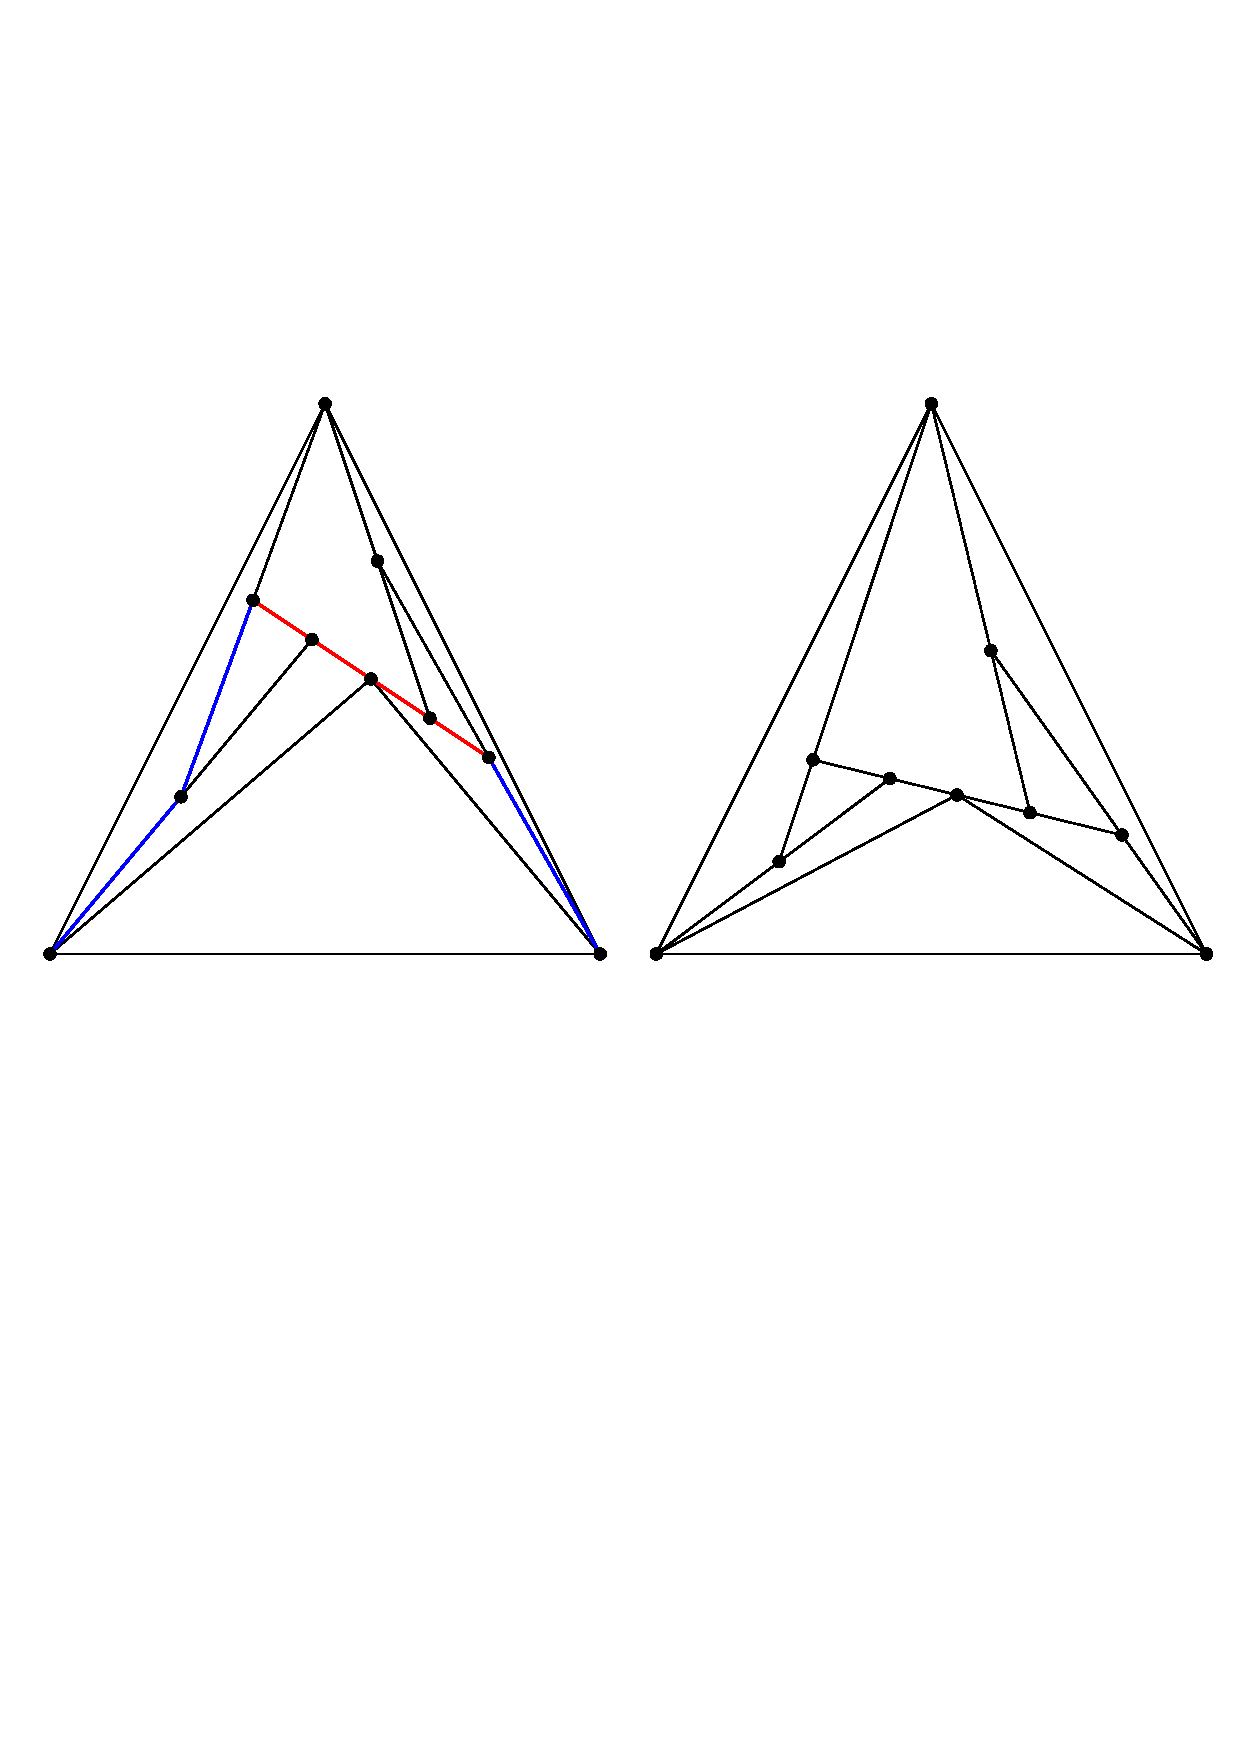
\includegraphics[width=1\textwidth]{example1_vis.pdf}
  \caption{Drei Zeichnungen der gleichen SLTR für unterschiedliche $\lambda$. a) Für $\lambda=1$. b) Nach dem Ansatz aus Beispiel \ref{bsp_long_segment}. c) Nach dem Ansatz aus Beispiel \ref{bsp_long_segment}.}
  \label{large_corner}
\end{figure}

\subsection{Eine heuristisch gute Wahl von $\lambda$}

Der Ansatz aus Beispiel \ref{bsp_large_corner} führt jedoch auch bei einigen Graphen zu unschönen Zeichnungen. Ein Kompromiss aus beiden, hat heuristisch vielversprechende Zeichnungen erzeugt. Wir führen die beiden Algorithmen hintereinander aus. Falls das Schema aus Beispiel \ref{bsp_long_segment} konvergiert, brechen wir ab und geben die Zeichnung aus. Falls nicht, speichern wir die berechneten Werte $\lambda'$ und führen das Schema aus Beispiel \ref{bsp_large_corner} durch. Bei jedem Schritt berechnen wir nun eine neue Zeichnung mit $\lambda(e) = \lambda_{i+1}(e) + \lambda'(e)$. Wieder führen wir 50 Schritte durch.  TODO

Beispiele von so errechneten Zeichnungen verschiedener SLTRs sind in Abbildung \ref{vis_examples} zu sehen.

\section{Experimentelle Rechnungen}\label{stats}

Es folgt eine kurze statistische Betrachtung der Verteilung von Graphen mit SLTRs. Hier würde eine gleichmäßige Wahl von (intern-)3-zusammenhängenden Graphen die aufschlussreichsten Resultate liefern. Ein Algorithmus zur zufälligen Erstellung 3-zusammenhängender planarer Graphen lässt sich zum Beispiel nach einem Ansatz von Fusy implementieren \cite{fusy09}. Als Teilschritt der Erstellung eines uniformen Samplers für planare Graphen werden hier 3-zusammenhängende planare Graphen mit gleichverteilter Wahrscheinlichkeit erzeugt. Die Implementierung ist jedoch aufgrund der notwendigen Auswertung von Erzeugendenfunktionen kompliziert. Diese Analyse beschränkt sich daher auf pseudo-zufällig erzeugte Graphen. 

Es folgt eine kurze Beschreibung des von uns benutzen Samplers. Wir beginnen mit $G_0 = K_4$. Nun wird in Schritt $i$ mit noch zu wählenden Wahrscheinlichkeiten eine der folgenden vier Operationen durchgeführt.

\begin{itemize}
\item[PG1] Ein Knoten $v$ mit deg$(v) \geq 4$ wird in $v_1,v_2$ geteilt und eine Kante $(v_1,v_2)$ eingefügt. Nun werden die zyklisch sortierten Nachbarn in zwei Teile $N_1,N_2$ getrennt und mit $v_1$ beziehungsweise $v_2$ verbunden.
\item[PG2] Eine Knoten wird auf einer Kante eingefügt und mit einem in einem angrenzenden Gebiet liegenden Knoten verbunden.
\item[PG3] Ein Knoten wird in ein Gebiet eingefügt und mit mindestens drei der am Gebiet liegenden Knoten verbunden. 
\item[PG4] Es wird eine zufällige Kante in ein Gebiet mit mehr als drei Knoten eingefügt.
\end{itemize}

Nach jeder dieser Operationen ist $G_i$ weiterhin planar und die Erzeugung kann bei der gewünschten Knotenzahl angehalten werden. Abschließend wird zufällig ein äußeres Gebiet und aus diesem die Aufhängungen gewählt. Die Parameter der pseudo-zufälligen Erzeugung sind durch drei aufsteigende natürliche Zahlen $(a,b,c)$, mit $a\leq b\leq c\leq 1000$, gegeben und lassen sich anpassen. In jedem Schritt wird eine der vier Möglichkeiten PG1, PG2, PG3 und PG4 mit Verteilung $a/1000$, $(a+b)/1000$, $(a+b+c)/1000$ und $(1000-a-b-c)/1000$ ausgewählt. Wir benutzen zur Gewinnung der statistischen Daten Werte, die sich um $(a,b,c) \approx (380,650,990)$ bewegen.


\begin{figure}
        \centering
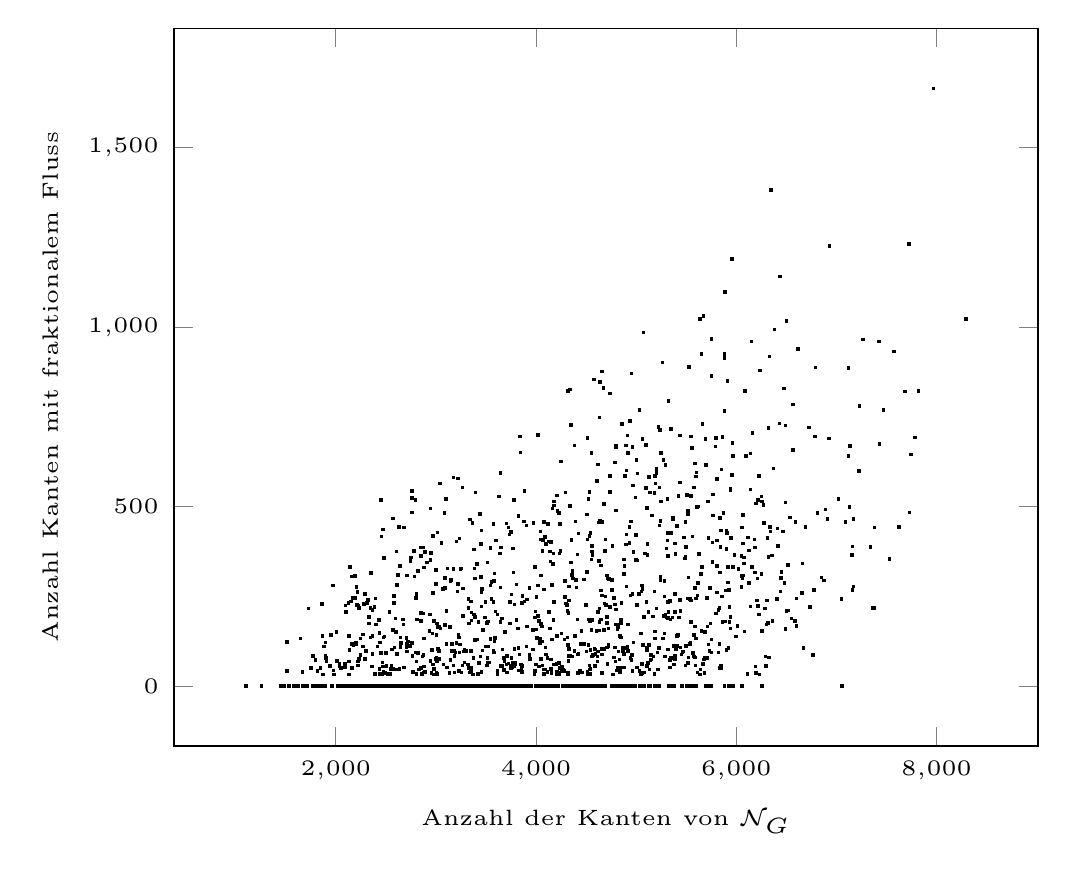
\begin{tikzpicture}[thick, scale=1.6,font=\tiny]
\begin{axis}[xlabel=Anzahl der Kanten von $\mathcal{N}_G$,ylabel=Anzahl Kanten mit fraktionalem Fluss]

\addplot[
	scatter/classes={
    	s={mark=square*,scale=0.1,black}
    	},
	scatter,only marks,
    	scatter src=explicit symbolic,]
	table[meta=label] {
x y label
4207 531 s
3768 383 s
3475 0 s
3682 78 s
4031 182 s
3433 64 s
4632 749 s
4241 451 s
4178 235 s
3945 0 s
3839 695 s
4674 831 s
3375 78 s
4577 854 s
3534 66 s
4165 495 s
4043 431 s
4388 139 s
3772 66 s
3821 161 s
4534 541 s
4066 377 s
4511 478 s
4381 0 s
4515 408 s
4596 90 s
4167 340 s
3814 0 s
4246 376 s
4453 154 s
4630 348 s
5100 672 s
4382 671 s
4848 136 s
3991 42 s
3884 236 s
4393 459 s
4566 366 s
4656 877 s
3658 56 s
4801 670 s
4680 508 s
4741 540 s
4368 300 s
4337 0 s
3561 0 s
4878 353 s
4998 421 s
4791 623 s
4552 650 s
4638 847 s
5063 689 s
4741 816 s
4300 230 s
4047 308 s
4567 86 s
4954 871 s
4398 296 s
4327 238 s
5032 770 s
4608 571 s
4896 670 s
5202 594 s
4693 408 s
4231 36 s
4996 351 s
4718 300 s
4216 0 s
4935 443 s
4759 296 s
5379 0 s
4535 419 s
5225 722 s
4257 53 s
4620 206 s
4636 462 s
4764 390 s
4962 667 s
4912 698 s
4209 139 s
4851 174 s
4698 226 s
5753 864 s
4422 425 s
4038 120 s
3823 44 s
5182 264 s
4291 249 s
4019 0 s
4214 488 s
4544 427 s
4738 542 s
4129 206 s
4100 0 s
5011 593 s
4224 34 s
4946 459 s
5071 985 s
4689 376 s
4617 617 s
5247 650 s
4722 160 s
4991 526 s
5059 280 s
5235 553 s
5249 515 s
4813 158 s
5639 1023 s
5193 564 s
5674 1031 s
5187 586 s
4632 216 s
5136 539 s
5158 475 s
4034 0 s
4680 156 s
5232 448 s
4524 521 s
5663 731 s
4515 40 s
5528 889 s
5005 630 s
5304 384 s
5518 478 s
4664 458 s
5751 967 s
5047 147 s
5240 713 s
5599 584 s
5245 460 s
5311 522 s
4905 423 s
5559 664 s
4891 586 s
4597 0 s
5441 209 s
4543 34 s
4529 186 s
5184 538 s
5285 250 s
5342 186 s
4852 232 s
5881 915 s
4683 103 s
4904 0 s
5693 689 s
5387 257 s
5724 116 s
4413 38 s
5882 926 s
5106 56 s
5507 532 s
5370 465 s
4314 210 s
5685 80 s
5850 604 s
5549 695 s
5319 426 s
5385 206 s
5885 1099 s
5614 252 s
6151 961 s
6181 408 s
4880 52 s
4418 0 s
5619 287 s
5496 111 s
6329 918 s
5295 616 s
4787 228 s
4146 0 s
5957 589 s
5808 577 s
5652 925 s
5809 406 s
5860 694 s
4514 34 s
4953 73 s
5388 398 s
5440 698 s
6379 994 s
6346 1382 s
5311 406 s
5485 356 s
6434 1141 s
5837 316 s
5699 616 s
5492 361 s
5061 270 s
6567 785 s
5964 678 s
5767 476 s
6357 364 s
6501 1017 s
5968 641 s
6723 721 s
6614 939 s
5437 568 s
5597 132 s
5919 289 s
1971 280 s
1767 0 s
2162 118 s
2333 193 s
2099 225 s
2041 0 s
2221 224 s
2323 240 s
2206 276 s
1861 229 s
2218 262 s
2177 114 s
2094 62 s
2211 226 s
2199 246 s
2366 140 s
2507 0 s
2402 0 s
2264 0 s
1896 84 s
1513 42 s
2053 0 s
2139 0 s
2275 0 s
2186 0 s
2231 218 s
2273 110 s
2441 122 s
2145 332 s
2039 55 s
2311 232 s
2470 436 s
2430 184 s
1875 32 s
1864 0 s
2233 76 s
2306 0 s
2367 212 s
2400 172 s
2389 221 s
2712 308 s
2319 0 s
2631 443 s
2346 136 s
2076 0 s
2480 357 s
2877 386 s
2564 0 s
2797 518 s
2202 120 s
2611 282 s
2509 56 s
2443 34 s
2623 310 s
2597 188 s
2759 524 s
2243 0 s
2853 386 s
2642 334 s
2460 0 s
3009 174 s
2762 543 s
2535 206 s
2741 112 s
2565 0 s
2953 371 s
2766 84 s
3040 565 s
2416 0 s
2418 110 s
2811 0 s
2780 377 s
2940 200 s
3178 581 s
3008 38 s
2558 58 s
2799 245 s
2548 48 s
2969 260 s
2171 0 s
2585 108 s
2947 495 s
2882 54 s
2814 0 s
2852 204 s
2754 359 s
2934 154 s
2808 256 s
2969 418 s
3086 483 s
2670 186 s
2822 321 s
2812 186 s
2737 0 s
2770 40 s
3219 578 s
3237 411 s
2385 0 s
2544 34 s
3408 340 s
3265 554 s
2645 136 s
3107 210 s
3019 165 s
2853 181 s
3056 399 s
3217 264 s
3073 270 s
2883 38 s
3324 243 s
3099 522 s
3393 192 s
3449 396 s
3161 118 s
3364 454 s
3286 66 s
3091 274 s
3424 178 s
3246 327 s
3352 236 s
3007 142 s
3093 171 s
3133 0 s
2714 0 s
3048 161 s
3518 180 s
3024 96 s
3178 327 s
3354 50 s
3023 104 s
3581 94 s
3547 131 s
3420 34 s
3703 453 s
3249 0 s
3089 301 s
3394 539 s
2851 52 s
3029 98 s
3660 189 s
3451 304 s
3457 262 s
3275 0 s
3240 116 s
3338 464 s
2860 0 s
3269 272 s
3257 38 s
3207 120 s
3547 280 s
3214 0 s
3045 160 s
3520 0 s
3709 0 s
3933 274 s
3463 270 s
3575 452 s
3514 345 s
3705 60 s
3544 385 s
4019 700 s
3355 205 s
3307 98 s
3217 0 s
3741 174 s
3904 447 s
4098 396 s
3709 84 s
3577 234 s
3725 442 s
3455 0 s
3805 283 s
3881 459 s
3627 0 s
3912 241 s
3885 544 s
3685 68 s
4292 539 s
3613 200 s
3775 0 s
3993 208 s
3990 332 s
3442 480 s
4247 626 s
3976 455 s
3774 316 s
3598 406 s
4045 409 s
4319 822 s
4337 826 s
4070 407 s
4177 503 s
3652 386 s
4337 502 s
3738 234 s
3751 429 s
3792 0 s
4125 403 s
3186 38 s
3593 208 s
4206 62 s
3516 0 s
1454 0 s
1894 0 s
1885 110 s
1620 0 s
2051 50 s
1830 0 s
1720 0 s
1773 84 s
2179 0 s
2271 144 s
1899 122 s
1727 216 s
1106 0 s
2163 50 s
1669 40 s
1692 0 s
1810 0 s
2269 0 s
2209 116 s
1908 68 s
1669 0 s
1951 142 s
2178 0 s
2349 218 s
1258 0 s
1903 78 s
2127 231 s
2150 236 s
2458 417 s
1848 50 s
2190 307 s
1895 0 s
2010 70 s
2131 68 s
2574 467 s
2395 244 s
1810 0 s
2221 68 s
1887 0 s
1675 0 s
2682 442 s
2452 519 s
2334 174 s
2293 257 s
2246 132 s
2202 0 s
2175 0 s
2218 0 s
2583 251 s
2675 172 s
2131 32 s
2303 98 s
2759 484 s
2655 0 s
2313 0 s
2132 0 s
2438 148 s
2468 66 s
2464 0 s
2435 0 s
1960 0 s
2498 38 s
2185 0 s
2522 34 s
2247 0 s
2303 0 s
2853 363 s
2270 0 s
2601 46 s
2337 0 s
2298 0 s
2163 0 s
1940 56 s
2351 315 s
2570 156 s
2880 330 s
2967 146 s
3014 428 s
2041 0 s
2448 0 s
2438 48 s
2479 0 s
2471 54 s
2091 53 s
2595 0 s
2484 0 s
2684 52 s
3089 0 s
2197 0 s
2391 34 s
2943 0 s
2996 76 s
1528 0 s
2089 0 s
2368 90 s
2019 0 s
2980 182 s
3059 0 s
2417 0 s
2705 109 s
2762 120 s
2448 0 s
2500 0 s
2584 231 s
3002 323 s
2341 0 s
2234 0 s
2746 0 s
2192 0 s
2803 94 s
2501 92 s
2256 0 s
2647 109 s
2840 0 s
2501 0 s
2946 70 s
3406 0 s
2876 202 s
2890 40 s
3043 0 s
2785 306 s
2891 374 s
2478 136 s
3646 275 s
2722 124 s
2614 90 s
3152 295 s
3222 284 s
2380 0 s
3116 328 s
2778 0 s
3380 381 s
2290 76 s
2475 40 s
2223 58 s
2835 0 s
2524 0 s
3148 291 s
2853 50 s
3325 218 s
2574 48 s
2601 150 s
3647 594 s
2642 0 s
2443 0 s
2790 0 s
2716 0 s
3844 651 s
2832 0 s
3329 174 s
3033 0 s
3780 0 s
3195 94 s
2753 0 s
3134 36 s
3387 328 s
3748 58 s
2946 0 s
2971 60 s
3287 102 s
2710 96 s
3584 314 s
3454 222 s
3236 94 s
3145 72 s
2883 132 s
2829 46 s
3583 124 s
3207 403 s
3251 0 s
2712 119 s
2982 48 s
2984 0 s
3509 58 s
2490 36 s
3354 183 s
2450 92 s
2866 82 s
3226 0 s
2721 0 s
3685 0 s
2859 34 s
4351 727 s
3408 130 s
2035 0 s
3556 243 s
3781 519 s
2823 0 s
3088 0 s
3466 99 s
3639 0 s
3180 98 s
2653 120 s
3445 82 s
3825 474 s
4020 280 s
3077 60 s
3784 228 s
2691 0 s
3724 63 s
3865 251 s
3367 0 s
4182 515 s
4120 452 s
3451 0 s
2291 0 s
3266 0 s
3555 290 s
3508 0 s
3562 0 s
3620 0 s
3147 0 s
3498 0 s
4008 134 s
3690 150 s
3861 232 s
4365 321 s
3342 38 s
2577 0 s
3516 78 s
2423 0 s
4138 375 s
2874 0 s
3999 60 s
3861 56 s
3295 0 s
2487 0 s
4041 130 s
4175 369 s
4515 692 s
3343 0 s
3992 191 s
3737 0 s
3273 0 s
4016 0 s
3940 76 s
2973 0 s
4174 184 s
3112 52 s
4353 407 s
3647 178 s
4331 278 s
4288 293 s
4314 136 s
4137 160 s
3267 0 s
2639 0 s
3396 0 s
3349 98 s
4692 250 s
3469 156 s
3997 158 s
3795 62 s
4087 415 s
4311 226 s
3844 0 s
2972 0 s
4004 248 s
2961 0 s
3356 52 s
4558 82 s
4477 297 s
4048 173 s
2913 0 s
3853 48 s
4146 347 s
5263 902 s
3968 156 s
4416 367 s
4432 0 s
4556 353 s
3287 0 s
3644 56 s
4233 369 s
3455 0 s
4161 282 s
4227 34 s
5115 396 s
4499 226 s
4940 739 s
3026 0 s
3159 98 s
5271 630 s
3454 40 s
4966 559 s
4114 78 s
4090 0 s
4136 0 s
3711 38 s
4155 36 s
4317 114 s
4077 269 s
4911 106 s
4537 182 s
4031 54 s
3806 184 s
3616 42 s
3106 117 s
4756 268 s
4725 116 s
4360 310 s
4725 110 s
4801 490 s
4076 46 s
4326 70 s
3621 0 s
3756 78 s
3203 0 s
4120 0 s
4885 334 s
2452 0 s
5189 152 s
5350 716 s
2565 0 s
4275 0 s
3588 134 s
4208 34 s
3517 66 s
3827 106 s
4707 192 s
4899 394 s
4160 130 s
3646 0 s
3005 0 s
4731 298 s
3752 50 s
3526 110 s
3789 0 s
4871 106 s
4059 124 s
3904 110 s
5244 295 s
4113 40 s
3457 0 s
4397 0 s
3985 32 s
2821 0 s
4590 56 s
4935 399 s
3469 0 s
4659 252 s
3598 0 s
5109 497 s
5241 305 s
2211 0 s
4565 184 s
5955 1191 s
4178 60 s
4460 38 s
5066 114 s
4500 0 s
4823 96 s
4229 64 s
5316 362 s
5549 239 s
5350 427 s
4768 32 s
3497 110 s
4093 108 s
3769 0 s
3348 40 s
4651 267 s
5205 0 s
5546 530 s
4286 130 s
5439 240 s
4209 40 s
5421 530 s
5606 499 s
4634 178 s
4364 82 s
4903 278 s
4595 102 s
4614 68 s
4785 0 s
5130 582 s
4647 336 s
4217 0 s
3784 104 s
4683 230 s
3680 46 s
3562 0 s
5009 350 s
5391 368 s
3168 0 s
3545 0 s
4995 0 s
3667 102 s
4889 0 s
5030 256 s
6226 585 s
4816 50 s
3710 0 s
4126 0 s
4558 0 s
5760 346 s
4606 153 s
4609 0 s
4477 118 s
6237 879 s
5617 500 s
5601 595 s
%% So far we have 4 graphs each between 100 and 300.
2101 207 s
2170 246 s
2023 0 s
2161 305 s
1512 123 s
1483 0 s
1585 0 s
1717 0 s
2134 140 s
2023 0 s
1872 0 s
1869 140 s
1961 0 s
1790 0 s
1797 72 s
1752 50 s
1624 0 s
2197 0 s
1977 44 s
2076 0 s
2213 0 s
2085 0 s
2268 0 s
2592 0 s
2415 0 s
2007 150 s
2226 0 s
2280 229 s
2357 0 s
1818 42 s
1769 0 s
2098 0 s
2607 375 s
2083 0 s
2138 100 s
2036 0 s
2300 0 s
2105 0 s
2485 138 s
1648 133 s
2257 0 s
2076 0 s
2464 34 s
2645 0 s
2247 86 s
1532 0 s
2745 349 s
2945 352 s
2261 0 s
2038 63 s
1885 0 s
2963 100 s
2911 345 s
2808 68 s
2806 34 s
2562 102 s
3199 0 s
2455 0 s
1984 32 s
1781 0 s
3002 284 s
3031 166 s
3007 78 s
2364 54 s
3143 164 s
3392 300 s
2812 0 s
3252 328 s
2035 0 s
2637 48 s
2883 0 s
3013 68 s
2820 92 s
3275 96 s
2996 0 s
3629 528 s
2227 0 s
3495 234 s
3273 196 s
3229 42 s
3382 200 s
1689 0 s
2631 0 s
3029 76 s
1712 0 s
3642 370 s
3228 142 s
3491 191 s
3011 34 s
2587 0 s
4227 483 s
3457 433 s
3734 423 s
3187 84 s
2586 0 s
2345 0 s
3655 0 s
2380 0 s
2819 0 s
3656 0 s
3753 255 s
2907 0 s
4091 46 s
3402 0 s
3954 0 s
3373 32 s
3285 0 s
2708 134 s
3771 64 s
3594 0 s
3451 0 s
2064 0 s
3580 293 s
2957 36 s
4857 731 s
2975 32 s
4080 457 s
4736 586 s
3063 0 s
3423 0 s
4799 667 s
3168 0 s
4021 195 s
4152 402 s
2881 0 s
3390 128 s
3433 0 s
3792 66 s
4903 601 s
3614 34 s
4325 204 s
3291 0 s
2878 86 s
4921 649 s
3013 0 s
4254 147 s
3265 58 s
4162 0 s
3494 0 s
4508 318 s
3741 0 s
3233 135 s
3970 102 s
4561 390 s
4347 344 s
5324 794 s
3711 0 s
3861 40 s
3604 0 s
4944 253 s
3176 58 s
2177 0 s
5205 605 s
4554 156 s
3934 86 s
4707 308 s
3450 0 s
3573 98 s
3182 0 s
4560 375 s
4043 132 s
5320 190 s
3141 0 s
3031 0 s
4804 0 s
4536 46 s
3431 0 s
4413 0 s
3509 176 s
4881 312 s
5038 0 s
4450 117 s
3327 50 s
4737 220 s
4654 104 s
4584 0 s
4962 257 s
3834 88 s
5496 387 s
4404 275 s
4879 108 s
3616 0 s
4651 185 s
4797 214 s
2994 0 s
3635 0 s
5493 458 s
4185 0 s
5520 488 s
4848 184 s
3910 166 s
5106 107 s
3787 56 s
5405 446 s
4833 74 s
4973 373 s
4349 0 s
5126 114 s
4405 0 s
3315 0 s
4061 166 s
4418 36 s
3075 0 s
5122 206 s
5054 264 s
4914 110 s
4098 88 s
6086 823 s
5882 767 s
5795 691 s
4707 108 s
2605 0 s
4712 62 s
5561 417 s
5766 534 s
5903 100 s
3285 0 s
3178 0 s
3634 0 s
3945 0 s
4779 245 s
3165 0 s
4945 78 s
3862 0 s
3593 0 s
3371 0 s
6160 706 s
3286 0 s
3888 0 s
5323 206 s
4327 104 s
6259 514 s
5268 132 s
5124 0 s
4374 0 s
3274 0 s
3954 0 s
4791 108 s
6195 509 s
4269 0 s
4149 74 s
3123 0 s
6274 454 s
6293 83 s
5290 82 s
5917 332 s
5113 366 s
5350 79 s
6412 439 s
4957 86 s
5370 468 s
6199 36 s
4964 42 s
4973 122 s
5706 246 s
4314 0 s
4870 96 s
5524 80 s
5202 216 s
3884 0 s
5589 620 s
6477 829 s
6157 332 s
6142 648 s
3138 0 s
5943 545 s
4019 0 s
6211 300 s
5909 426 s
5098 552 s
4794 68 s
6931 1226 s
4627 0 s
4005 0 s
5007 52 s
4442 0 s
6565 658 s
6094 642 s
4664 0 s
4260 42 s
5418 142 s
5088 370 s
3599 0 s
4368 0 s
4049 76 s
6270 504 s
5309 191 s
4063 58 s
3535 0 s
3678 45 s
4526 114 s
5049 34 s
5138 0 s
5566 92 s
5932 179 s
6447 302 s
5649 312 s
5476 414 s
4424 89 s
5614 38 s
5169 194 s
3852 60 s
4754 0 s
5874 482 s
5594 58 s
3151 0 s
6340 431 s
4081 0 s
3763 52 s
4499 0 s
3688 0 s
6493 726 s
4079 34 s
4689 0 s
5185 34 s
5367 0 s
6055 442 s
3475 0 s
5521 303 s
5588 80 s
5956 0 s
7118 642 s
4806 44 s
6208 238 s
4971 0 s
6257 154 s
5809 261 s
3354 0 s
4140 0 s
3770 0 s
7225 599 s
5902 434 s
5848 56 s
5031 42 s
4918 172 s
5587 274 s
4005 0 s
6053 362 s
5390 74 s
3459 0 s
5709 78 s
5847 434 s
5940 192 s
3653 0 s
5722 0 s
4094 0 s
5190 132 s
5211 94 s
6590 457 s
4609 0 s
6064 477 s
5596 0 s
5319 234 s
5831 218 s
5794 668 s
4202 0 s
7267 966 s
5820 94 s
4584 104 s
5730 98 s
3330 0 s
4536 58 s
4450 0 s
4840 0 s
4519 0 s
5229 106 s
4834 42 s
4940 0 s
4338 84 s
5530 0 s
5397 103 s
5807 335 s
6059 307 s
5565 0 s
5174 82 s
3834 0 s
3628 0 s
6517 211 s
6218 519 s
5904 382 s
4778 0 s
4384 0 s
4498 0 s
3740 0 s
4508 0 s
5843 388 s
4317 38 s
5593 0 s
6851 303 s
6335 444 s
6406 243 s
5887 180 s
5922 106 s
5547 178 s
5050 0 s
5930 220 s
5378 112 s
6113 34 s
5083 0 s
6775 268 s
7022 522 s
5750 130 s
4946 0 s
6076 342 s
6415 391 s
4971 0 s
6190 54 s
4576 0 s
5148 86 s
4784 0 s
3871 0 s
3764 0 s
4116 0 s
5638 32 s
6662 342 s
5377 60 s
4842 42 s
6370 606 s
5658 332 s
5861 178 s
4542 0 s
4544 48 s
5032 0 s
7158 268 s
5319 102 s
5579 142 s
4290 0 s
4793 172 s
5643 46 s
6297 56 s
5295 199 s
3726 0 s
5736 273 s
4534 0 s
5678 74 s
6553 188 s
6311 412 s
6890 492 s
5362 191 s
6763 87 s
4660 36 s
4427 0 s
6449 318 s
4434 0 s
3908 0 s
3719 0 s
3832 0 s
8291 1023 s
5457 0 s
6784 696 s
5337 237 s
5324 0 s
5043 38 s
7049 243 s
6226 200 s
6254 0 s
6363 182 s
7379 442 s
5212 0 s
4977 0 s
5084 38 s
5748 0 s
5129 0 s
4312 0 s
5753 94 s
5232 0 s
5330 0 s
7531 354 s
5226 0 s
6185 386 s
5974 0 s
5597 244 s
4917 98 s
3574 0 s
5144 72 s
5275 196 s
4540 0 s
4546 0 s
7627 444 s
5151 74 s
4957 0 s
7136 669 s
3903 0 s
3860 0 s
6655 260 s
4280 42 s
5218 46 s
4840 140 s
5035 0 s
4115 0 s
7376 217 s
4264 0 s
3341 0 s
7730 484 s
6600 244 s
6492 159 s
5540 118 s
7817 823 s
6081 152 s
4297 0 s
7687 821 s
5839 469 s
5913 850 s
3577 0 s
4629 456 s
4878 90 s
3875 0 s
5941 550 s
5339 72 s
6124 288 s
4383 98 s
4817 170 s
4470 0 s
5409 139 s
6252 529 s
4074 0 s
3171 0 s
5441 107 s
4619 96 s
4708 176 s
5966 332 s
6429 732 s
5076 193 s
5340 52 s
5184 0 s
4817 163 s
6216 223 s
3333 0 s
3902 0 s
6071 308 s
4533 0 s
6252 312 s
4080 0 s
5510 0 s
4287 0 s
4635 155 s
5006 226 s
4052 0 s
3993 0 s
4502 96 s
5282 293 s
4148 48 s
6140 548 s
3717 0 s
4168 0 s
4610 0 s
4414 186 s
5580 554 s
3437 0 s
5535 243 s
5451 88 s
3808 0 s
5197 0 s
5107 101 s
4055 0 s
6315 176 s
5715 514 s
3480 0 s
3931 0 s
5945 413 s
5761 400 s
3280 0 s
3038 0 s
5689 150 s
4849 52 s
5997 138 s
6321 719 s
5506 0 s
5120 64 s
5984 365 s
4920 96 s
6116 414 s
6492 512 s
6078 358 s
2890 0 s
4273 46 s
5710 166 s
4480 0 s
4876 0 s
4544 100 s
4972 0 s
5465 96 s
4482 0 s
5283 147 s
5102 235 s
4317 34 s
5941 161 s
6327 80 s
5884 0 s
4318 34 s
4083 0 s
4237 50 s
6285 216 s
4616 82 s
6876 294 s
7726 1232 s
6064 397 s
7425 960 s
4838 40 s
5822 212 s
5388 84 s
3381 0 s
3770 0 s
6584 182 s
4439 42 s
4152 0 s
5796 202 s
5429 191 s
3648 0 s
6789 888 s
5724 413 s
7121 887 s
4670 0 s
7161 389 s
6480 288 s
5579 82 s
6736 220 s
6465 431 s
5588 166 s
4932 0 s
4059 0 s
6516 338 s
6537 470 s
6304 238 s
7131 499 s
6909 466 s
6232 32 s
4593 0 s
4370 0 s
7969 1666 s
4012 0 s
5743 174 s
5513 244 s
5833 50 s
6928 690 s
5464 94 s
7230 781 s
3039 0 s
4661 88 s
5195 0 s
5625 368 s
7092 457 s
4328 84 s
6811 483 s
4487 0 s
5665 62 s
6690 444 s
6441 264 s
5056 36 s
5412 112 s
6063 302 s
7428 674 s
6501 210 s
6023 327 s
5849 50 s
7364 217 s
5927 268 s
6011 168 s
7468 770 s
4778 80 s
6052 276 s
7056 0 s
5896 267 s
7577 933 s
4541 0 s
6322 360 s
5682 36 s
7155 365 s
4550 0 s
6600 168 s
6303 172 s
6142 222 s
5341 0 s
7168 278 s
5493 58 s
6186 316 s
7339 388 s
7742 646 s
4555 0 s
5833 117 s
3322 60 s
5920 0 s
7170 466 s
6126 378 s
4071 0 s
5544 122 s
6059 0 s
3920 0 s
4759 0 s
5855 250 s
4415 88 s
3704 0 s
5058 62 s
3561 0 s
5695 0 s
5519 64 s
4637 0 s
7784 693 s
5653 154 s
6673 106 s
5134 46 s
    };
\end{axis}
\end{tikzpicture}
\caption{ Ergebnisse von experimentellen Rechnungen des Programms auf pseudo-zufälligen planaren 3-zusammenhängenden Graphen mit SLTRs zur Veranschaulichung des fraktionalen Anteils der errechneten Lösungen.}
\label{table}
\end{figure}



In Abbildung \ref{table} sind die Ergebnisse für so erzeugte Graphen zwischen 100 und 1000 Knoten dargestellt, mit jeweils fünf Graphen pro Knotenanzahl. Ein Punkt in der Abbildung entspricht einem Graphen. Die Farben stehen für eine SLTR (blau), nur ein FAA (rot) oder einen Graphen mit keinem von beiden (grün). 
Wie nicht anders zu erwarten, bilden die Farben drei Strahlen, die sich mit wachsender Knotenzahl zunehmend vermischen. Die Parameter des Samplers wurden so gewählt, um gerade an diesem Übergang viele Graphen zu erzeugen. Für Graphen mit im Verhältnis großen Kantenzahlen finden sich fast immer SLTRs und für Graphen mit wenigen Kanten existieren nur selten FAAs.

Da wir uns am Ende von Kapitel \ref{main_algo} ausführlich mit nicht-ganzzahligen Lösungen beschäftig haben, wollen wir auch zu diesen eine statistische Einordnung vornehmen. In Abbildung \ref{non_int_table} ist eine solche zu sehen. Hier entspricht jeder Punkt einem zulässigen Fluss auf einem Netzwerk $\mathcal{N}_G$ zu unterschiedlichen Graphen $G$. Die Koordinaten entsprechen der der Kantenanzahl\footnote{Hierbei werden Kanten mitgezählt, die in einer zulässigen Lösung immer gesättigt oder in diesem Fall leer sind.} von $\mathcal{N}_G$ und der Kantenanzahl des fraktionalen Flusses. Insgesamt wurden jeweils die Lösungen für fünf Graphen mit SLTRs auf 100 bis 300 Knoten dargestellt. Es wurde erneut der oben beschriebene Sampler genutzt.

Wie wir sehen, werden oft ganzzahlige Lösungen zurück gegeben, selbst wenn wir nicht auf Ganzzahligkeit bestehen. Hinzu kommt, dass der Anteil des fraktionalen Flusses oft relativ klein ist.


\section{Dokumentation}

Zum Abschluss des Kapitels folgt eine Dokumentation des Programs. Die Datei \texttt{program.sage} muss in SageMath geladen werden \cite{sage}. Die beiden in \texttt{program.sage} implementierten Funktionen sind:
\begin{description}
\item[\texttt{sltr(graph, face, suspensions, non\char`_int, check\char`_int, plotting, ipe)}] \hfill \\
Gibt, falls möglich, ein Gutes-FAA zurück und erstellt optional eine Zeichnung.
\begin{description}
\item[\texttt{return = GFAA :}] Eine Gutes-FAA als Liste von Gebieten mit Zuweisungen, \texttt{[[[1,4,6,8],[4]], ... ]}, oder \texttt{None}.
\item[\texttt{graph :}] Ein planarer intern-3-zusammenhängender Graph
\item[\texttt{face :}] Das äußere Gebiet als Kantenfolge \texttt{[[$v_1,v_2$], ... ,[$v_k,v_1$]]}, mit \texttt{None} werden alle möglichen äußeren Gebiete überprüft.
\item[\texttt{suspensions :}] Die Aufhängungen als Liste \texttt{[$a_1,a_2,a_3$]}, mit \texttt{None} werden alle möglichen Aufhängungen überprüft. Falls ein äußeres Gebiet übergeben wurde müssen auch die Aufhängungen übergeben werden.
\item[\texttt{non\char`_int :}] default \texttt{True}, sonst wird nur nach ganzzahligen Lösungen gesucht.
\item[\texttt{check\char`_int :}] default \texttt{True}, sonst wird die Überprüfung ab Zeile \ref{algo_check} ausgelassen.
\item[\texttt{plotting :}] default \texttt{False}, sonst wird eine Zeichnung ausgegeben.
\item[\texttt{ipe :}] default \texttt{None}, bei Übergabe eines Strings \texttt{string} wird eine ipe-Datei \texttt{string.ipe} erstellt.
\end{description}
\item[\texttt{random\char`_sltr(vertices, non\char`_int, check\char`_int, plotting, ipe, cut)}] \hfill \\
Es wird ein pseudo-zufälliger Graph generiert und, falls möglich, ein Gutes-FAA zurückgegeben. Optional kann eine Zeichnung ausgegeben werden.
\begin{description}
\item[\texttt{return = [graph,GFAA]}] Ein Paar aus Graph und GFAA oder \texttt{[graph,None]}.
\item[\texttt{vertices :}] Die Anzahl der Knoten des zu erzeugenden Graphen
\item[\texttt{non\char`_int :}] default \texttt{True}, sonst wird nur nach ganzzahligen Lösungen gesucht.
\item[\texttt{check\char`_int :}] default \texttt{True}, sonst wird die Überprüfung ab Zeile \ref{algo_check} ausgelassen.
\item[\texttt{plotting :}] default \texttt{True}, sonst wird keine Zeichnung ausgegeben.
\item[\texttt{ipe :}] default \texttt{None}, bei Übergabe eines Strings \texttt{string} wird eine ipe-Datei \texttt{string.ipe} erstellt.
\item[\texttt{cut :}] default \texttt{None}, optional lassen sich die Parameter der pseudo-zufälligen Erzeugung durch drei aufsteigende natürliche Zahlen \texttt{[a, b, c]} anpassen, mit $a\leq b\leq c\leq 1000$. Es wird der in Abschnitt \ref{stats} beschriebene Sampler genutzt. Die normale Einstellung ist \texttt{[300,600,990]}. In jedem Schritt wird eine der vier Möglichkeiten PG1, PG2, PG3 und PG4 mit Verteilung $a/1000$, $(a+b)/1000$, $(a+b+c)/1000$ und $(1000-a-b-c)/1000$ ausgewählt.
\end{description}
\end{description}

